\documentclass[9pt]{beamer}

% \usepackage{etoolbox}
% \makeatletter
% Insert [short title] for \section in ToC
% \patchcmd{\beamer@section}{{#2}{\the\c@page}}{{#1}{\the\c@page}}{}{}
% Insert [short title] for \section in Navigation
% \patchcmd{\beamer@section}{{\the\c@section}{\secname}}{{\the\c@section}{#1}}{}{}
% Insert [short title] for \subsection in ToC
% \patchcmd{\beamer@subsection}{{#2}{\the\c@page}}{{#1}{\the\c@page}}{}{}
% Insert [short title] for \subsection  in Navigation
% \patchcmd{\beamer@subsection}{{\the\c@subsection}{#2}}{{\the\c@subsection}{#1}}{}{}
% \makeatother

\usepackage[utf8]{inputenc}
\usepackage{tikz-cd}
\usepackage{parskip}
\setlength{\parskip}{\medskipamount}
\makeatletter
\newcommand{\@minipagerestore}{\setlength{\parskip}{\medskipamount}}
\makeatother
\usefonttheme{serif}
\usetheme{miir}

\theoremstyle{definition}
\newtheorem{dfn}{Definition}[section]
\newtheorem{exl}[dfn]{Example}

\theoremstyle{plain}
\newtheorem{lem}[dfn]{Lemma}
\newtheorem{thm}[dfn]{Theorem}
\newtheorem{cor}[dfn]{Corollary}

\theoremstyle{remark}
\newtheorem{rmk}[dfn]{Remark}
\newtheorem*{claim}{Claim}

\newcommand\N{\ensuremath{\mathbb{N}}} % natural numbers
\newcommand\Z{\ensuremath{\mathbb{Z}}} % integers
\newcommand\Q{\ensuremath{\mathbb{Q}}} % rationals
\newcommand\R{\ensuremath{\mathbb{R}}} % real numbers
\newcommand\C{\ensuremath{\mathbb{C}}} % complex numbers

\newcommand\Half{\mathbb{H}} % half-plane
\newcommand\D{\ensuremath{\mathbb{D}}} % disc
\newcommand\fatou{\ensuremath{\mathcal{F}}} % fatou set
\newcommand\julia{\ensuremath{\mathcal{J}}} % julia set
\newcommand\kulia{\ensuremath{\mathcal{K}}} % filled julia set
\newcommand\nhd{\ensuremath{\mathcal{N}}} % neighbourhood 
\newcommand\basin{\ensuremath{\mathcal{A}}} % basin
\newcommand\petal{\ensuremath{\mathcal{P}}} % petal
\newcommand\kettle{\ensuremath{\mathcal{Q}}} % kettle
\newcommand\inv{^{-1}} % inverse

\newcommand\iter[2]{#1^{\circ#2}} % iterates of a map
\newcommand\inviter[2]{\iter{\left(#1\inv\right)}{#2}} %invorb
\newcommand\minuset{\ensuremath{-}} % set difference
\newcommand\tendsto{\longrightarrow}
\newcommand\abs[1]{\ensuremath{\left|#1\right|}}
\newcommand\norm[1]{\ensuremath{\|{#1}}\|}
\newcommand\cl[1]{\ensuremath{\overline{#1}}} % top closure
\newcommand\eps{\ensuremath{\varepsilon}} % standard epsilon

\newcommand\fix{z^*}          % fixed point
\newcommand\crit{z^{\#}}      % critical point
\newcommand\linT{\phi}        % linearization
\newcommand\linV{\psi}        % linearization the other way
\newcommand\lin[1]{           % linearized version
    \ensuremath{\hat{#1}}}    
\newcommand\LinT{\Phi}        % linearization near infty
\newcommand\LinV{\Psi}        % ditto 
\newcommand\Lin[1]{           % ditto 
    \ensuremath{\hat{#1}}}    
\newcommand\TrT{\omega}       % substitution
\newcommand\Tr[1]{            % substituted version
    \ensuremath{\tilde{#1}}}
\newcommand\sector{           % sector of the complex plane
    \ensuremath{\Delta}}
    \newcommand{\chart}{\zeta} % charts

\title{Local Normal Forms of Analytic Maps Near Fixed Points}
\author{
    [CID -- 01515432] Yuze Jin\newline 
    [CID -- 01514289] Anagh Malik\newline 
    [CID -- 01492068] Abhimanyu Pallavi Sudhir\newline
    [CID -- 01520955] Harmeet Singh\newline
    [CID -- 01227888] Jean (Chia-Chun) Lo\newline 
    {---}\newline
    \textbf{Supervisor}: Davoud Cheraghi}
\institute{Imperial College London}
\date{\today}

\begin{document}

% title
\titleframe
% toc
\begin{frame}{Outline}
\tableofcontents
\end{frame}

% content
% COMMENTING OUT FOR A BIT, COMPILATION IS TAKING FOREVER
% and also everyone else is like, done, anyway
\section{Introduction}
\begin{frame}{Introducion}
    \begin{itemize}
        \item $f : \nhd \tendsto \C$ analytic function
        \item $z^* \in \nhd$ fixed point $f(z^*) = z^*$
        \item Forward orbit
        \[
        \mathcal{O}(z) := \left\{z, f(z), \iter{f}{2}(z), \dots, \iter{f}{n}(z), \dots \right\}
        \]
        \[
        \iter{f}{n} = \underbrace{f \circ f \circ \dots f \circ f}_\text{$n$}
        \]
        \item Conjugating by local biholomorphism $\phi$
        \[
        \phi \circ f \circ \phi^{-1}
        \]
    \end{itemize}
\end{frame}

\begin{frame}{Introduction}
    \begin{itemize}
        \item Since conjugation preserves dynamics, we assume fixed point is at the origin
        \item $\lambda = f'(0)$ is called the multiplier and is invariant under conjugation
        \item $z \in \nhd$ is a \emph{periodic point with period $q$} of $f$ if $\iter{f}{q}(z) = z$ and $\iter{f}{(q+1)}(z) \neq z$
        % i need to know stuff about your presentation
        % pls help
    \end{itemize}
\end{frame}
\section{Geometrically Attracting or Repelling Fixed Points}
\sectiontitleframe

\begin{frame}{Topologically attracting}
    \begin{definition}The fixed point $\fix$ of $f$ is    called \emph{topologically attracting} if\,   $\exists$\, a neighbourhood $U$ on which the iterates ${f}^{\circ n}$ are defined and converge uniformly to the constant map $z \longmapsto z^*$.
    \end {definition}
\end{frame}    
    
\begin{frame}{Topologically attracting and multiplier }
  
        \begin{theorem}
          Consider the function $f(z)=\lambda z+a_{2} z^{2}+a_{3} z^{3}+\dots$ with fixed point $z^*=0$. Then the origin is topologically attracting iff $\abs{\lambda}<1$.
        \end{theorem}
 
       

\end{frame}
\begin{frame}{Koenigs linerisation}
    \begin{theorem}
    For $ f(z)=\lambda z+a_{2} z^{2}+a_{3} z^{3}+\dots$ such that $\abs{\lambda} \notin \{0,1\}$, there exists a local biholomorphic function $\lin{z}=\linT(z)$ in some neighbourhood $\nhd$ of 0 such that the following diagram commute and $\linT (0)=0$ 
    \begin{figure}
    \centering
    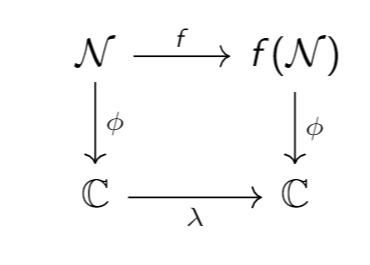
\includegraphics[width=3cm]{resources/ch-08/graph1.png}
   
    \end{figure}

    \end{theorem} 
    Here $ \linT(z)=\lim _{n \tendsto \infty} \iter{f}{n}(z) / \lambda^{n}$
\end{frame}


                    
          

\begin{frame}{Basin of attraction}
    \begin{definition}
        \label{intro:dfn:basin}
        The \emph{attraction basin} $\basin$ of a fixed point $z^*$ is the set of all points that converge to $z^*$ under iterations of $f$
        \begin{equation*}
            \basin(z^*) = \{z_0\mid \lim_{n \rightarrow \infty} \iter{f}{n}(z_0) = z^*\}
        \end{equation*}
        The \emph{immediate basin} $\basin_0$ is the connected component of $\basin$ that contains $z^*$.
    \end{definition}
\end{frame}
\begin{frame}{Global linearisation for a geometrically attracting fixed point}
    \begin{theorem}[Global linearisation] 
        \label{8:thm:attlinglob}
        Up to multiplication by a non-zero constant, there exists a unique local biholomorphic map $\linT:\basin\to\C$ such that the following diagram commute and $\linT(0)=0$.
    \end{theorem}
 
     \begin{figure}
    \centering
    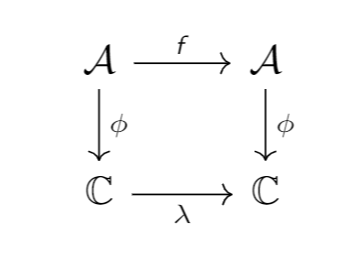
\includegraphics[width=3cm]{resources/ch-08/graph2.png}
    \end{figure} 
    
    We can prove this by defining $\linT(z)=\lambda^{-n}\linT_r(\iter{f}{n}(z))$ where $n$ is the smallest integer for which $\abs{\iter{f}{n}(z)}<r$.
\end{frame}

\begin{frame}{Inverse of linearization and critical point}
    In this lemma consider $f$ is a rational function with degree $\geq 2$ over $\widehat{\C}$ and the fixed point $\fix \in \mathbb{C}$ so that the local behaviour is exactly the same as before.
    \begin{lemma}
    The local inverse in the last theorem $\linV_\eps: \D_{\eps} \to \basin_{0}$ can be uniquely analytically extended to some maximal open disc $\D_{r}$ as $\linV_r: \D_{r} \to \basin_{0}$ with $\linV_r(0)=0$ and $\linT\circ \linV_r(\lin{z}) = \lin{z}$. 
    
    Furthermore, $\linV_r$  can be continuously extended to the boundary $\partial \D_{r}$ and there exists at least one critical point of $f$ in the $\linV_r(\partial \D_{r})$.
    \end{lemma}
\end{frame}

\begin{frame}{Attracting periodic orbit}
    \begin{definition}

        A \emph{periodic orbit} is an orbit $z_0 \rightarrow z_1 \rightarrow z_2 \rightarrow \cdots $ such that $z_m =\iter{f}{m}(z_0)=z_0$ for some integer $m$. A periodic orbit is called \emph{attracting} if the derivative $\abs{\left(\iter{f}{m}\right)'\left(z_{k}\right)}<1$. 
    \end{definition}
    
    Note:  $\abs{\left(\iter{f}{m}\right)'\left(z_{k}\right)}$ is the same for all $z_{k}$.
    
    \begin{definition}
    Since each $z_k$ is a fixed point of $\iter{f}{m}$, they have corresponding immediate basins. The immediate basin $\basin_0(\mathcal{O}, f)$ of a periodic orbit $\mathcal{O}$ is the union of the immediate basins of each point in the orbit under $\iter{f}{m}$.
    \end{definition}
    
\end{frame}

\begin{frame}{Attracting periodic orbit and critical point}
    \begin{theorem}
        For $f$ a nonlinear rational map, the immediate basin of every attracting periodic orbit contains at least one critical point.
    \end{theorem}
    
    Idea of proof: 
    
    \begin{itemize}
        \item $f^{\circ m}$ maps $\basin^{0}\left(z_{j}\right)$ into itself. 
        \item $f$ has no critical point $\implies f^{\circ m}$ no critical point.
        \item Basin of attraction of a attracting fixed point must contain a critical point.
    \end{itemize}
\end{frame}
\begin{frame}{Approximating attracting periodic orbit}
    \begin{cor}
    \label{8:cor:orbfin}
    Such a rational map $f$ has only finitely many attracting periodic orbits.
    \end{cor}   
    
    \textbf{A logarithm for approximating periodic orbit:} 
    
    \begin{itemize}
        \item Locate all critical points of the function
        \item Iteratively apply the function from the critical point.
        \item Observe if it converges to a periodic orbit.
    \end{itemize}
    
    \textbf{Note}: May fail for large period. e.g.$f(z)=z^2-1.5$.
\end{frame}

\begin{frame}{Topologically Repelling}
    \begin{definition}
   
    The fixed point $\fix$ of $f$ is called \emph{topologically repelling} if for some neighbourhood $\nhd$ of $\fix$, $\forall z \in \nhd $ and $z \neq \fix,\; \exists\, n \in \N$ s.t. $\iter{f}{n}\left(z\right)$ leaves $\nhd$.  Here we call $\nhd$ a \emph{forward isolating neighbourhood} of $\fix$.
    \end{definition}
    
    \textbf{Note}: The only orbit that stays in $\nhd$ is the orbit of the fixed point $\fix$.
\end{frame}

\begin{frame}{Topologically repelling and multiplier}
    \begin{theorem}
          Consider the function $f(z)=\lambda z+a_{2} z^{2}+a_{3} z^{3}+\dots$ with fixed point $z^*=0$. Then the origin is topologically repelling iff $\abs{\lambda}>1$.
        \end{theorem}
\end{frame}

\begin{frame}{generlization of $\linV_{\epsilon}$ in repelling case}
    \begin{thm}
    For a repelling fixed point of $f$, there exists an entire bijective function $\linV$ such that $\linV (0)=0$ and $\linV$ conjugates $f$ to the linear map $\lin{z} \mapsto \lambda\lin{z}$. Moreover, $\linV$ is unique (up to multiplication by a non-zero constant).
     \begin{figure}
    \centering
    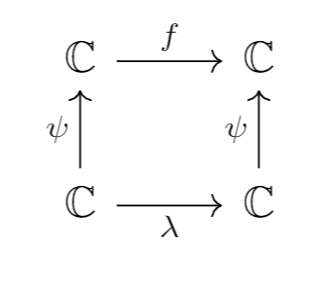
\includegraphics[width=3cm]{resources/ch-08/graph3.png}
   
    \end{figure}
    \end{thm} 
   
   \textbf{Idea of proof}: 
   
   Choose the smallest $n$  such that $z/{\lambda ^{n}}\in\D_{\eps}(0)$, then define $\linV(z)=\iter{f}{n}(\linV_{\eps} (z/{\lambda ^{n}}))$.
\end{frame}

\section{Superattracting Fixed Points}
\sectiontitleframe

\begin{frame}{Introduction}

    \begin{definition}
    A holomorphic function $f : \C \rightarrow \C$ has a super-attracting fixed point at $z^* \in \C$, if $f(z^*)=z^*$ and $f'(z^*) = 0$.
    \end{definition}\bigskip
    
    WLOG fixed point at 0, we can write:
    
    \begin{equation}
    \label{9:eq:1}
    f(z) = a_pz^p + a_{p+1}z^{p+1}\dots = \sum_{k=p}^{\infty} a_{k}z^k
    \end{equation}
    
\end{frame}


\begin{frame}{Bottcher's Theorem}

\begin{thm}
    \label{9:thm:bottcher}
    Let $f$ be as in Eq.~\ref{9:eq:1}. Then there exists a local holomorphic change of coordinates $\lin{z} = \linT(z)$, such that $\linT(0) = 0$ and $\linT'(0) = 1$, where $\linT(f(z)) = \phi(z)^p$ locally. Furthermore, $\linT$ is unique up to multiplication by a $(p-1)^{th}$ root of unity. 
\end{thm}
\medskip
    
    \begin{itemize}
        \item existence and uniqueness of map $\phi : \C \rightarrow \C$
        \item $\linT(f(z)) = \phi(z)^p$
        \item derivative at 0 is 1
        \item existence of inverse $\psi$
        \item $\phi \circ f \circ \phi^{-1} (z) = z^p$
        
    \end{itemize}
    
\end{frame}




\begin{frame}{Inverse of the change of coordinates}

\begin{thm}
\label{9:thm:extension}
Let $f$ and $\linT$ be as in Theorem \ref{9:thm:bottcher} and let $\linV_r$ be local inverse of $\phi$. Then there exists a unique open disc $\D_\eps$ around 0 of maximal radius $0<\eps \leq 1$ such that $\linV_r$ extends holomorphically to a map $\linV$ from the disc into the immediate basin $\basin^0$ of $0$. If $\eps=1$, then $\linV$ maps the unit disc biholomorphically onto $\basin^0$ and $0$ is the only critical point of f in the basin. On the other hand if $\eps<1$ then there is at least one other critical point of $f$ in $\basin^0$, lying on the boundary of $\linV(\D_\eps)$.
\end{thm}\bigskip
    
    \begin{itemize}
        \item Holomorphic extension of $\psi$, to:
        \begin{enumerate}
            \item Another critical point, $\psi$ valid on $\D_\eps$, critical point on boundary of image of $\D_\eps$ under the map $\psi$.
            
            \item No other critical point, $\psi$ biholomorphism from $\D_1$ to immediate basin.
        \end{enumerate}

    \end{itemize}
    
\end{frame}



\begin{frame}{First Example}

\begin{exl}

Take:

$$f(z) = \frac{z^2}{1-2z^2} \approx z^2+2z^4+4z^6\dots$$


By our Theorem \ref{9:thm:extension} the extension of the inverse of the map valid in whole of $\D_1$. Inverse given by:


$$\linV(\lin{z}) = \frac{\lin{z}}{1+\lin{z}^2}$$

We then see:

$$f(\linV(\lin{z})) = f\left(\frac{\lin{z}}{1+\lin{z}^2}\right) = \frac{\lin{z}^2}{1+\lin{z}^4} = \linV(\lin{z}^2)$$
\end{exl}
    
\end{frame}


\begin{frame}{Applications to Polynomial Dynamics}
    Now we will be working on the Riemann Sphere, let:
    \begin{equation}
f(z) = a_dz^d + a_{d+1}z^{d+1}\dots+a_1z + a_0
\end{equation}

\begin{itemize}
    \item WLOG we can assume f to be monic
    \item super-attracting fixed point at $\infty$
\end{itemize}
\end{frame}


% \begin{frame}{Application to Polynomial Dynamics}

% \begin{dfn}
% We call the set of all $z \in \widehat{\C}$ with a bounded orbit under f the \emph{filled Julia set} of f, $\kulia = \kulia(f)$. 
% \end{dfn}

% \begin{thm}
% \label{9:thm:1.6}
% For any polynomial $f$ of degree at least 2, the filled Julia set $\kulia \subset \widehat{\C}$ is compact, with connected complement and with $\partial \kulia = \julia = \julia(f)$ (the Julia set) and with interior equal to the union of all the bounded components $U$ of the Fatou set $\widehat{\C}\setminus\julia$. Thus $K$ is equal to the union of all such $U$ and $\julia$ itself. 
% \end{thm}

    
% \end{frame}

\begin{frame}{Fixed point at $\infty$}
Let $\zeta = \frac{1}{z}$. Then:

$$G(\zeta) = \frac{1}{f(1/\zeta)}$$

Then since $f$ is monic, near $\infty$, $f(z) \approx z^d$. By that we have near 0, $$G(\zeta) \approx \frac{1}{z^d} = \zeta^d$$

Then from Theorem \ref{9:thm:bottcher} we can get a map $\alpha$, which conjugates $G$ to $\Lin{z} \mapsto \Lin{z}^d$. Let:

$$\linT(z) = \frac{1}{\alpha(\frac{1}{z})}$$

which maps some neighbourhood of $\infty$ biholomorphically onto another neighbourhood of $\infty$. We then have:

$$\linT(f(z)) = \linT(z)^d$$

\end{frame}

\begin{frame}{Example}

    \begin{exl}
Let's take the map:

$$f(z) = z^2 -2$$ 

Super-attracting fixed point at $\infty$. Let $\zeta = 1/z$ and get map $G(\zeta)$:

$$G(\zeta) = \frac{1}{f\left(\frac{1}{\zeta}\right)} = \frac{\zeta^2}{1-2\zeta^2}$$

For $G$ we had the local inverse $\beta(\Lin{z}) = \frac{\Lin{z}}{1+\Lin{z}^2}$, here we have:

$$\linV(\lin{z}) = \frac{1}{\beta(1/\lin{z})} = \lin{z} +\frac{1}{\lin{z}}$$

For verification we find:

$$f\left(\lin{z} + \frac{1}{\lin{z}}\right) = \lin{z}^2 + \frac{1}{\lin{z}^2} = \linV(\lin{z}^2)$$


\end{exl}

\end{frame}
\section{Parabolic Fixed Points}
\sectiontitleframe

\begin{frame}{Attraction vectors}
    \begin{equation*}
        f(z)=\lambda z + \mu z^{p + 1} + \dots
    \end{equation*}
    \begin{itemize}
        \item When $\lambda = 1$, fixed point exhibits both attractive and repulsive properties.
        \item Consider wanting for $\alpha\in\R^+$ (\emph{non-constant}),  $f(\eps)=\alpha\eps$, i.e. an infinitesimal vector on which $f$ acts as scaling. 
        \item For $\lambda = 1$, this has solutions $\eps^p=(\alpha - 1)/\mu$
        \begin{itemize}
            \item \emph{attraction vectors} $v_-^p = -1/(p\mu)$
            \item \emph{repulsion vectors} $v_+^p = +1/(p\mu)$
        \end{itemize}
        \item $v_j = v_0\exp(j/p\cdot \pi i)$ repulsion for even $j$, attraction for odd $j$.
    \end{itemize}
\end{frame}
\begin{frame}{Attraction vectors}
    \begin{figure}
        \centering
        \begin{tikzpicture}[x=0.75pt,y=0.75pt,yscale=-1,xscale=1]
%uncomment if require: \path (0,235); %set diagram left start at 0, and has height of 235

%Straight Lines [id:da7014467597216401] 
\draw    (334,128.64) -- (431.9,128.29) ;
\draw [shift={(434.9,128.28)}, rotate = 539.79] [fill={rgb, 255:red, 0; green, 0; blue, 0 }  ][line width=0.08]  [draw opacity=0] (8.93,-4.29) -- (0,0) -- (8.93,4.29) -- cycle    ;
%Straight Lines [id:da7937079638414151] 
\draw    (334,128.64) -- (284.43,44.86) ;
\draw [shift={(282.9,42.28)}, rotate = 419.39] [fill={rgb, 255:red, 0; green, 0; blue, 0 }  ][line width=0.08]  [draw opacity=0] (8.93,-4.29) -- (0,0) -- (8.93,4.29) -- cycle    ;
%Straight Lines [id:da5652322657720215] 
\draw    (334,128.64) -- (282.51,209.74) ;
\draw [shift={(280.9,212.28)}, rotate = 302.40999999999997] [fill={rgb, 255:red, 0; green, 0; blue, 0 }  ][line width=0.08]  [draw opacity=0] (8.93,-4.29) -- (0,0) -- (8.93,4.29) -- cycle    ;
%Straight Lines [id:da49795176320656886] 
\draw    (384.9,42.28) -- (335.52,126.05) ;
\draw [shift={(334,128.64)}, rotate = 300.51] [fill={rgb, 255:red, 0; green, 0; blue, 0 }  ][line width=0.08]  [draw opacity=0] (8.93,-4.29) -- (0,0) -- (8.93,4.29) -- cycle    ;
%Straight Lines [id:da9443327330326834] 
\draw    (233.9,128.28) -- (331,128.63) ;
\draw [shift={(334,128.64)}, rotate = 180.21] [fill={rgb, 255:red, 0; green, 0; blue, 0 }  ][line width=0.08]  [draw opacity=0] (8.93,-4.29) -- (0,0) -- (8.93,4.29) -- cycle    ;
%Straight Lines [id:da7066291127526734] 
\draw    (385.1,215) -- (335.53,131.22) ;
\draw [shift={(334,128.64)}, rotate = 419.39] [fill={rgb, 255:red, 0; green, 0; blue, 0 }  ][line width=0.08]  [draw opacity=0] (8.93,-4.29) -- (0,0) -- (8.93,4.29) -- cycle    ;
%Curve Lines [id:da8961728852679585] 
\draw    (351.9,124.28) .. controls (472.29,125.27) and (412.51,10.81) .. (349.84,113.71) ;
\draw [shift={(348.9,115.28)}, rotate = 300.82] [fill={rgb, 255:red, 0; green, 0; blue, 0 }  ][line width=0.08]  [draw opacity=0] (8.93,-4.29) -- (0,0) -- (8.93,4.29) -- cycle    ;
%Curve Lines [id:da6878104068351576] 
\draw    (327.9,109.28) .. controls (273.17,12.15) and (394.67,12.65) .. (338.76,107.83) ;
\draw [shift={(337.9,109.28)}, rotate = 300.98] [fill={rgb, 255:red, 0; green, 0; blue, 0 }  ][line width=0.08]  [draw opacity=0] (8.93,-4.29) -- (0,0) -- (8.93,4.29) -- cycle    ;
%Curve Lines [id:da6213553894464128] 
\draw    (319.9,113.28) .. controls (261.19,19.13) and (195.56,120.63) .. (312.13,121.27) ;
\draw [shift={(313.9,121.28)}, rotate = 539.81] [fill={rgb, 255:red, 0; green, 0; blue, 0 }  ][line width=0.08]  [draw opacity=0] (8.93,-4.29) -- (0,0) -- (8.93,4.29) -- cycle    ;
%Curve Lines [id:da5023612601796306] 
\draw    (319.9,143.28) .. controls (257.21,240.17) and (196.51,136.7) .. (315.1,134.3) ;
\draw [shift={(316.9,134.28)}, rotate = 539.3399999999999] [fill={rgb, 255:red, 0; green, 0; blue, 0 }  ][line width=0.08]  [draw opacity=0] (8.93,-4.29) -- (0,0) -- (8.93,4.29) -- cycle    ;
%Curve Lines [id:da5020349766396639] 
\draw    (329.9,144.28) .. controls (273.18,245.15) and (389.72,245.66) .. (338.68,145.79) ;
\draw [shift={(337.9,144.28)}, rotate = 422.4] [fill={rgb, 255:red, 0; green, 0; blue, 0 }  ][line width=0.08]  [draw opacity=0] (8.93,-4.29) -- (0,0) -- (8.93,4.29) -- cycle    ;
%Curve Lines [id:da4534345213536044] 
\draw    (350.9,132.28) .. controls (469.3,134.65) and (411.49,244.55) .. (347.86,141.84) ;
\draw [shift={(346.9,140.28)}, rotate = 418.73] [fill={rgb, 255:red, 0; green, 0; blue, 0 }  ][line width=0.08]  [draw opacity=0] (8.93,-4.29) -- (0,0) -- (8.93,4.29) -- cycle    ;
\end{tikzpicture}

        \caption{Attraction and repulsion vectors, basins where $p = 3$, $\mu\in\R^{> 0}$}
    \end{figure}
\end{frame}
\begin{frame}{Attraction vectors}
    This intuition is formalized in the following results.
    \newline
    \begin{thm}
        Let $f$ be a holomorphic function as with $\lambda = 1$. Let $z_0$ be such that the sequence $z_n=\iter{f}{n}(z_0)\tendsto 0$ but $\forall n, z_n\ne 0$. Then, for some attraction vector $v_j$ satisfying $v_j^p=-1/(p\mu)$,
        \begin{equation*}
            \lim_{n\tendsto\infty} n^{1/p} z_n = v_j
        \end{equation*}
        i.e. $z_n\sim v_j/n^{1/p}$ asymptotically. $z_n$ is said to tend to 0 \emph{in the direction of $v_j$}.
    \end{thm}
    \begin{cor}
        Let $z_0$ be such that the sequence $z_n=\inviter{f}{n}(z_0)\tendsto 0$ but $\forall n, z_n\ne 0$. Then, for some repulsion vector $v_j$ of $f$ satisfying $v_j^p = 1/(p\mu)$, $z_n\sim v_j/n^{1/p}$.
    \end{cor}
\end{frame}
\begin{frame}{Rotational parabolic points}
    We have sneakily been setting $\lambda = 1$. The following result justifies ``WLOG $\lambda = 1$''.\newline
    \begin{dfn}
        Let $v$ be a complex number.  
        \begin{itemize}
            \item If there exists a sequence $z_n=\iter{f}{n}(z_0)\tendsto 0$ (but $\forall n, z_n\ne 0$) with a subsequence $z_{n_k}$ such that $\arg z_{n_k}\tendsto\arg v$, then $v$ is called an attraction vector for $f$.
            \item If there exists a sequence $z_n=\inviter{f}{n}(z_0)\tendsto 0$ (but $\forall n, z_n\ne 0$) with subsequence $z_{n_k}$ such that $\arg z_{n_k}\tendsto\arg v$, then $v$ is called an repulsion vector for $f$.
        \end{itemize}
    \end{dfn} 
    \begin{thm}
        The attraction vectors of $f$ are the same as the same as those of $\iter{f}{r}$, and their number is a multiple of $r$.
    \end{thm}
\end{frame}
\begin{frame}{Attraction basins}
    \begin{itemize}
        \item A specialized ``directional'' notion of an attraction basin is thus needed for our purposes.
        \item Similarly, the notion of a \emph{petal} acts as a directional notion of a neighbourhood of a fixed point.
    \end{itemize}
\end{frame}
\begin{frame}{Basins and petals}
    \begin{dfn}
        The basin of attraction $\basin_v$ for an attraction vector $v$ is defined as the set of points $z$ such that $\iter{f}{n}(z)\tendsto 0$ in the direction of $v$. The immediate basin of attraction $\basin_v^0$ is defined as the unique connected component of $\basin_v$ that is closed under $f$.
    \end{dfn}
    \begin{dfn}
        Where $f$ is injective on some neighbourhood $\nhd$ of its fixed point, an open set $\petal \subseteq \nhd$ is called an attracting petal for $f$ along attraction vector $v$ if 
        \begin{enumerate} 
            \item $\petal$ is closed under $f$.
            \item $\petal\subseteq\basin_v$
            \item Any orbit $\iter{f}{n}(z_0)$ converging to 0 along $v$ is eventually in $\petal$. 
        \end{enumerate}
    \end{dfn}
\end{frame}
\begin{frame}{Basins and petals}
    Basic expected results on attraction basins and neighbourhoods transfer to our new definitions.
    \begin{lem}
        The attraction basin is open.
    \end{lem}
    \begin{lem}
        The basins of attraction $\basin_v$ are contained in the Fatou set of $f$, while their boundaries $\partial\basin_v$ are contained in the Julia set.
    \end{lem}
    \begin{lem}
    Where $f$ is a non-linear rational map with parabolic fixed point 0 and multiplier $\lambda = 1$: 
        \begin{enumerate}
            \item each immediate basin of 0 contains at least one critical point of $f$.
            \item each basin contains exactly one petal $\petal_\mathrm{max}$ that maps injectively onto some right half-plane under $\linT$ and is maximal with respect to this property. 
            \item $\petal_\mathrm{max}$ has at least one critical point of $f$ on its boundary.
        \end{enumerate}
    \end{lem}
\end{frame}
\begin{frame}{Abel linearization}
    \begin{itemize}
        \item $\linT(f(z))=\linT(z)$ is \emph{not} a local homeomorphism!
        \item Better idea to find a linearization: take inspiration from the ``inherent structure on the petal''. $\linT(f(z))=\linT(z)+1$.
    \end{itemize}
    \begin{thm}[Parabolic linearisation theorem]
        Given an attracting or repelling petal $\petal$, there exists a unique (up to composition on the left with translation) conformal embedding $\linT:\petal\to\C$ called a Fatou co-ordinate on $\petal$ such that, for all $z\in\petal\cup {f}\inv(\petal)$, we have:
        \begin{equation*}
            \linT(f(z))=\linT(z)+1
        \end{equation*}
    \end{thm}
\end{frame}
\begin{frame}{Abel linearization}
    \begin{itemize}
        \item Does not immediately suffice for a normal form
        \item Can ``paste'' linearization of each petal together -- Ecalle-Voronin classification
    \end{itemize}
\end{frame}
\section{Irrationally Indifferent Fixed Points}
\sectiontitleframe
%\sectiontitleframe{Cremer Points and Siegel Discs}

\subsection{Cremer's non-linearisation theorem}
\begin{frame}{Local Linearisation}
$\lambda = e^{2\pi i \xi}$ where $\xi \in [0,1)$ is irrational.
    \begin{dfn}[Locally linearisable] The function $f$ above is said to be \emph{locally linearisable} if there is a local biholomorphic map $\linV$ which conjugates $f$ to a linear map:
\begin{equation}\label{eq: Schroder}
    \left(\linV^{-1} \circ f \circ \linV\right)(z) = \lambda z, \;
\end{equation}
for all $z$ in some neighbourhood of the origin.
\end{dfn}
\end{frame}

\begin{frame}
  We say an irrationally indifferent fixed point is a \textit{Cremer point} if there is no local linearisation of $f$ around the fixed point. A connected component of the Fatou set on which f is conjugate to a rotation of the unit disc is called a \emph{Siegel disc}.
 \begin{figure}
    \label{8:fig:Siegel Disc}
    \centering
    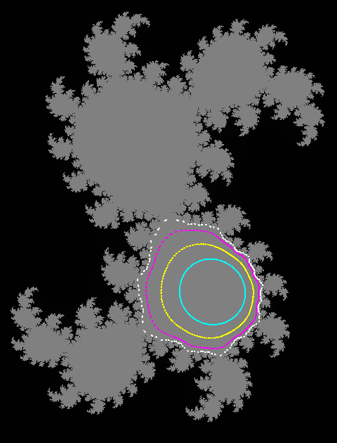
\includegraphics[width=4cm]{resources/ch-11/Picture1.png}
    \caption{Example of Siegel Disc, in white, in filled Julia set. Here, the cyan, yellow and magenta depict orbits of points nearby the origin} % <3
    
\end{figure}
\end{frame}

\begin{frame}
Main Theorems:
\begin{itemize}
    \item Cremer's Non-Linearisation Theorem
    \setbeamercovered{transparent}
    \item \onslide<2->{Siegel's Linearisation Theorem}
    \item \onslide<3->{Postcritical Closure}
\end{itemize}
\end{frame}

\begin{frame}{Cremer's Non-linearization Theorem}
    \begin{thm}(Cremer, 1938) \label{thm: 11.2}
    Given $\lambda \in \C$ on the unit circle and $d \geq 2$, if the sequence $\sqrt[d^{q}]{1 / \abs{\lambda^q - 1}}$ is unbounded as $q \tendsto \infty$, no fixed point with multiplier $\lambda$ of a rational function of degree $d$ can be locally linearisable.
\end{thm}
\end{frame}

\begin{frame}{Sketch Proof Cremer's Theorem}
Case when
\[
f(z) = z^{d} + \dots + \lambda z,  d \geq 2
\]
\begin{itemize}
    \item $f^{oq}(z) = z^{d^{q}} + \dots + \lambda^{q} z$
    \item Fixed points of $f^{oq}$ satisfy the polynomial $z^{d^{q}} + \dots + (\lambda^{q} - 1)z = 0$. Then 
    \[
    \prod_{j = 1}^{d^{q}-1} \left|{ z_{q}{(j)}}\right| = \abs{\lambda^{q} - 1}
    \]
    \item $\abs{\lambda^{q} - 1} < 1 \Longrightarrow \exists\; j_{q}$\; s.t.\;$ 0 < \left| z_{q}(j_q) \right| < \abs{\lambda^{q} - 1}^{1/d^{q}}$
    \item Sequence $(q_{k})_{k\geq 1}$ where
    \begin{align*}
    \abs{\lambda^{q_k} - 1}^{-1/d^{q_{k}}} &\tendsto \infty\\
    \implies \abs{\lambda^{q_k} - 1}^{1/d^{q_{k}}} &\tendsto 0
    \end{align*}
    \item Every neighbourhood of the origin has infinitely many periodic points
\end{itemize}
\end{frame}

\begin{frame}{Siegel's Linearization Theorem}
\begin{dfn}
For $\xi \in \R$, we say $\xi$ is \textit{Diophantine of order $\leq \kappa$} if\; $\exists\; \eps > 0$ such that
\[
\abs{\xi - \frac{p}{q}} > \frac{\eps}{q^{\kappa}}
\]
for any rational $\frac{p}{q}$
\end{dfn}

Certainly Diophantine of order $\leq \kappa \Longrightarrow$ Diophantine of order $\leq \kappa + 1$

\begin{lem}
With $\xi$ as above, $\xi$ is Diophantine of order $\leq \kappa \Longleftrightarrow$ there exists $M > 0$ such that $\forall\; q \in \Z_{\geq 1}$
\[
1/\abs{\lambda^{q}-1} < Mq^{\kappa - 1}
\]
\end{lem}
\end{frame}

\begin{frame}{Siegel's Linearization Theorem}
\begin{thm}
If the angle $\xi$ is Diophantine of any order, then any
holomorphic germ with multiplier $\lambda = e^{2\pi i\xi}$ is locally linearisable. Hence, if there exists $M > 0$ and $k \in \N$ such that $\forall\; q \in \Z_{\geq 1}$
\[
1/\abs{\lambda^{q}-1} < Mq^{k}
\]
then any holomorphic function with a fixed point of multiplier $\lambda$ is locally linearisale.
\end{thm}
\begin{cor}
In terms of the Lebesgue measure on $[0,1)$, almost every $\xi$ has the property that any holomorphic function with fixed point of multiplier $e^{2\pi i \xi}$ is locally linearizable. 
\end{cor}
\end{frame}

\begin{frame}{Generic vs Lebesgue Almost Everywhere}
    \begin{itemize}
        \item Cremer: for a \textit{generic} choice of angle $\xi$, there exists a holomorphic function with fixed point of multiplier $\lambda = e^{2\pi i \xi}$ which is not locally linearizable.
        \item Siegel: for \textit{almost every} angle $\xi$, any holomorphic function with fixed point of multiplier $\lambda = e^{2\pi i \xi}$ is locally linearizable.
    \end{itemize}
    
     \par\vspace{1em}
     
    \textit{A linguist would be shocked to learn that if a set is not closed this does not mean that it is open, or again that “E is dense in E” does not mean the same thing as “E is dense in itself"}
    
     \par\vspace{1em}
    % Yeah I latex
    % D:<
    - John Edensor Littlewood (1885–1977)
\end{frame}





















\newcommand\altfm[1][$\dagger$]{\textsuperscript{#1}}
\newcommand\altft[2][$\dagger$]{\footnotesize{\altfm[#1] #2}}
\newcommand\altfr{\vfill\rule{16em}{0.4pt}\par}
\newcommand\by[1]{\text{\footnotesize{(#1)}}}

\subsection{Siegel's Linearisation Theorem}
\begin{frame}{Siegel's Linearisation Theorem}
\begin{theorem}[Siegel 1942]
If $\xi$ is Diophantine of any order, then every germ of a holomorphic map with fixed point of multiplier $\lambda = e^{2\pi i\xi}$ is locally linearisable.
\end{theorem}\pause

\begin{theorem}[Quadratic Siegel discs exist]
For Lebesgue-almost all irrational $\lambda \in \R/\Z$, $f_\lambda(z) = \lambda z + z^2$ has a Siegel disc about the origin.
\end{theorem}

This is strictly weaker than Siegel (1942).
\end{frame}

\subsection{Siegel's Linearisation Theorem (Weak Version)}

\begin{frame}
\begin{thm}[Riemann mapping theorem]
Let $U \subset \C$ be a simply connected domain. Then for every $z_0 \in U$ there is a unique conformal isomorphism $\phi: U \to \D$ to the unit disc such that
\[
\phi(z_0) = 0 \quad\text{and}\quad \phi'(z_0) > 0
\]
\end{thm}
\pause
\begin{dfn}[Conformal radius] The \emph{conformal radius} of $U$ as viewed from $z_0 \in U$ is $\operatorname{rad}(U, z_0) = \dfrac{1}{\phi'(z_0)}$.
\end{dfn}
\pause
\emph{Intuition:} requiring instead $\phi: U \to \D_r$ with $\phi'(0) = 1$:
\[
\begin{tikzcd}[ampersand replacement=\&]
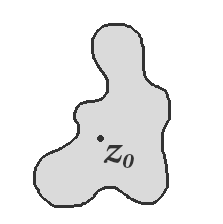
\includegraphics[width=0.2\textwidth]{resources/ch-11/uniformisation-blob.png}
\ar[r, "\phi",
start anchor={[yshift=.08\textwidth]},
end anchor={[yshift=.08\textwidth]}] \&
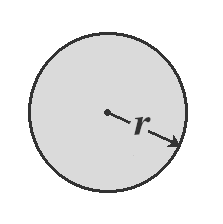
\includegraphics[width=0.2\textwidth]{resources/ch-11/uniformisation-circle.png}
\end{tikzcd}
\]
\end{frame}

\begin{frame}
    \begin{dfn}[Conformal radius function]
    For $\lambda \in \C$, let $\sigma(\lambda)$ be the conformal radius from $0$ of the maximal neighbourhood about $0$ on which $f_\lambda$ is conjugate to a rotation.
    
    \pause
    If no such neighbourhood exists, set $\sigma(\lambda) = 0$.
    \end{dfn}
    \pause

    Some properties:
    \begin{itemize}
        \item $\sigma$ is non-constant ($\sigma(0) = 0$, $\sigma(\lambda) > 0$ for $\abs{\lambda} \notin \{0, 1\}$.)
        \item $\sigma$ is \emph{upper semi-continuous} on $\cl{\D}$. 
    \end{itemize}
    
\end{frame}

\begin{frame}
\begin{itemize}
    \item When $\abs{\lambda} < 1$, Koenigs linearisation:
\end{itemize}

\[
\begin{tikzcd}[ampersand replacement=\&]
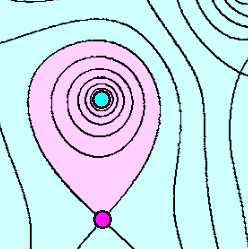
\includegraphics[width=0.2\textwidth]{resources/ch-11/julia-attracting-local.png}
\ar[r, "\phi",
start anchor={[yshift=.08\textwidth]},
end anchor={[yshift=.08\textwidth]}] \&
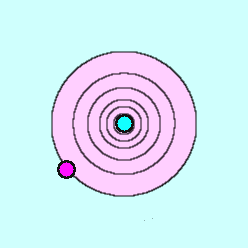
\includegraphics[width=0.2\textwidth]{resources/ch-11/julia-circle.png}
\end{tikzcd}
\]

\pause
\begin{itemize}
    \item $\eta(\lambda) = \phi({\color{magenta}-\lambda/2})$. The function $\eta(\lambda)$ is holomorphic on the punctured disc. The singularity at the origin is removable --- have $\sigma(\lambda) = \abs{\eta(\lambda)}$ on $\D$.
    \pause \item Computation:
    \[
\eta(\lambda) = -\frac{\lambda}{4} + \frac{\lambda^2}{16}
+\frac{\lambda^3}{16} + \frac{\lambda^4}{32} + \frac{9\lambda^5}{256} + \frac{\lambda^6}{256} +
\frac{7\lambda^7}{256} + O(\lambda^8)
\]
\end{itemize}

\end{frame}

\begin{frame}
\begin{lem}[F. and M. Riesz, 1916]\label{lem:A.3}
    Let $\eta: \D \to \C$ be bounded and holomorphic. If for some constant $c \in \C$ the set of $\xi$ such that
    \[
    \lim_{r\nearrow 1} \eta (r e^{2\pi i \xi}) = c
    \]
    has positive Lebesgue measure, then $\eta$ is constant.
\end{lem}
\vspace{1em}
\pause

\begin{proof}[Proof (quadratic Siegel discs exist)]

$\displaystyle \phantom{=}\ \{ \xi \in \R/\Z \mid
   z \mapsto e^{2\pi i \xi} z + z^2 \text{ not linearisable at $z = 0$} \}$

$\displaystyle = \{ \xi \in \R/\Z \mid
    \sigma(e^{2\pi i \xi}) = 0 \}$ \hfill {\footnotesize(by definition of $\sigma$)}

$\displaystyle = \{ \xi \in \R/\Z \mid
    \lim_{r \nearrow 1} \eta(r e^{2\pi i \xi}) = 0 \} $ \hfill {\footnotesize(upper semi-continuity)}
    
is a set of Lebesgue measure zero.
\end{proof}
\end{frame}

% Stronk version

\subsection{Siegel's Linearisation Theorem}
\begin{frame}{Siegel's Linearisation Theorem}
Strong version.

\begin{theorem}[Siegel 1942]
If $\xi$ is Diophantine of any order, then every germ of a holomorphic map with fixed point of multiplier $\lambda = e^{2\pi i\xi}$ is locally linearisable.
\end{theorem}
\end{frame}

\begin{frame}
\emph{Schröder's equation:} given $f$, seek $\psi$ such that $f(\psi(z)) = \psi(\lambda z)$
\[
\begin{tikzcd}[ampersand replacement=\&]
\C \ar[r, "f"] \& \C\\
\D_r \ar[u, "\psi"] \ar[r, "w \mapsto \lambda w"'] \& \D_r \ar[u, "\psi"']
\end{tikzcd}
\]
\pause
Up to first order:
\begin{itemize}
    \item $\psi(z) = z + \Psi(z)$
    \item $f(z) = \lambda z + F(z)$
\end{itemize}

Attempt instead to solve $F(z) = \Psi(\lambda z) - \lambda\Psi(z)$:
\pause
\[
    \Psi_0(z) = \sum_{j=2}^\infty \frac{b_j}{\lambda^j - \lambda}z^j
\]
in which $b_j$ are coefficients of the series expansion $F(z) = \sum_{j=2}^\infty b_j z^j$.
\end{frame}


% BRUTE FORCE BECAUSE
\begin{frame}
\[
\begin{tikzcd}[ampersand replacement=\&]
\D_{r_0} \ar[r, "f_0 = f"] \&[12em] \C
\ar[d, "\psi_0\inv"]
\\
\D_{r_1} \ar[u, "\psi_0"]
\ar[r, "f_1 = \psi_0 \circ \inv f \circ \psi_0"]
\&{}
\\
{}\&{} \\
{}\&{} \\
{}\&{}
\end{tikzcd}
\]
\end{frame}
\begin{frame}
\[
\begin{tikzcd}[ampersand replacement=\&]
\D_{r_0} \ar[r, "f_0 = f"] \&[12em] \C
\ar[d, "\psi_0\inv"]
\\
\D_{r_1} \ar[u, "\psi_0"]
\ar[r, "f_1 = \psi_0 \circ \inv f \circ \psi_0"]
\&
\ar[d, "\psi_1\inv"]
\\
\D_{r_2} \ar[u, "\psi_1"]
\ar[r, "f_2 = \psi_1\inv \circ \psi_0 \circ \inv f \circ \psi_0 \circ \psi_1"]
\&
\ar[d, "\psi_2\inv"] \\
\vdots
\ar[u, "\psi_2"]
\&
\vdots\\
{}
\&
{}
\end{tikzcd}
\]
\end{frame}

\begin{frame}
\[
\begin{tikzcd}[ampersand replacement=\&]
\D_{r_0} \ar[r, "f_0 = f"] \&[12em] \C
\ar[d, "\psi_0\inv"]
\\
\D_{r_1} \ar[u, "\psi_0"]
\ar[r, "f_1 = \psi_0 \circ \inv f \circ \psi_0"]
\&
\ar[d, "\psi_1\inv"]
\\
\D_{r_2} \ar[u, "\psi_1"]
\ar[r, "f_2 = \psi_1\inv \circ \psi_0 \circ \inv f \circ \psi_0 \circ \psi_1"]
\&
\ar[d, "\psi_2\inv"] \\
\vdots
\ar[r, color=white, "\textit{\color{black}(hopefully)}"']
\ar[u, "\psi_2"]
\&
\vdots\\
\D_{r_\infty} \ar[r, "z \mapsto \lambda z"]
\&
\D_{r_\infty}
\end{tikzcd}
\]
\end{frame}

\begin{frame}
Analysis ensues:
\begin{itemize}
    \pause \item Diophantine: $1/\abs{\lambda^q - 1} < M q^\kappa$
    \begin{itemize}
        \item $\abs{F_n}, \abs{\Psi_n} \tendsto 0$ fast enough
        \item $f_n$ tends to $z \mapsto \lambda z$; $\psi_n$ becomes close to the identity.
    \end{itemize}
    \pause \item Carefully check:
    \begin{itemize}
        \item Each $\psi_k, \psi_k\inv$ well-defined.
        \item $r_\infty > 0$.
    \end{itemize}
\end{itemize}
\end{frame}

\subsection{The Postcritical Closure}
\begin{frame}
What do Siegel discs \emph{look like?} \uncover<1->{Compare results from previous sections:}
\begin{minipage}{0.6\textwidth}
\begin{itemize}
    \item<1-> \emph{Attracting fixed point}:
    \begin{itemize}
        \item at least one critical point in {\color<1>{cyan}basin of attraction}.
        \item at least one critical point on boundary of
        {\color<1>{magenta} maximal linearising domain}.
    \end{itemize}
    %
    \item<2-> \emph{Parabolic fixed point} with $\lambda = 1$: 
    \begin{itemize}
        \item at least one critical point in each {\color<2>{cyan}immediate basin.}
        \item at least one critical point on boundary of {\color<2>{magenta}maximal attracting petal}.
    \end{itemize}
    %
    \item<3-> \emph{Irrationally indifferent fixed point}:
    \begin{itemize}
        \item are there critical points on the boundary of Siegel discs?
        \uncover<4->{
        \emph{Sometimes.\altfm}
    \vfill
    \altfr\altft{
    Herman M. 1985.
    \textit{Are there critical points on the boundaries of singular domains?}
    Comm. Math. Phys., 99(4):593–612}}
    \end{itemize}
\end{itemize}
\end{minipage}\hfill
\begin{minipage}{0.4\textwidth}
\includegraphics<1>[width=\textwidth]{resources/ch-11/julia-attracting.png}%
\includegraphics<2>[width=\textwidth]{resources/ch-11/julia-cauliflower.png}%
\includegraphics<3->[width=\textwidth]{resources/ch-11/julia-cauliflower-gs.png}%
\end{minipage}

\end{frame}
\begin{frame}
    \begin{dfn} The \emph{postcritical closure} of $f$ is the topological closure of the forward orbit of the set of critical points:
    \[
    P(f) = \cl{\bigcup_{k > 0} \iter{f}{k}(V(f))}
    \]
    where
    \[
    V(f) = \{ z \in \hat{\C} \mid f'(z) = 0 \}
    \]
    \end{dfn}
    \pause
    \par\vspace{1em}
    Equivalently, $P(f)$ is the smallest forward-invariant closed set containing all critical values of $f$.
\end{frame}

\subsection{The Postcritical Closure}
\begin{frame}
\begin{thm}
Each of the following sets is contained within $P(f)$:
\begin{itemize}
    \pause\item all (super-)attracting periodic orbits of $f$.
    \pause\item all indifferent periodic orbits which lie within $\julia(f)$.
    \pause\item the boundary of every period of rotation domains.
\end{itemize}
\end{thm}
\pause
\begin{proof}[Sketch of proof]
If $\abs{P(f)} < 3$: special case. $f$ is conjugate to $z \mapsto z^{\pm d}$.

Assume $\abs{P(f)} \ge 3$. Equip $Q = \hat{\C}\setminus P(f)$ with the \emph{Poincaré metric;} apply the Schwarz-Pick lemma to show that $\iter{f}{k}$ expands distances on $Q$.
\end{proof}
\end{frame}


\newcommand\imageonlyframe[3][1.0]{
{\setbeamercolor{background canvas}{bg=black}
\setbeamercolor{caption name}{fg=white}
\setbeamercolor{normal text}{fg=white}
\begin{frame}
\vfill
\begin{figure}
\includegraphics[width=#1\textwidth]{#2}
\caption{#3}
\end{figure}
\end{frame}
}}

\imageonlyframe[0.7]{resources/ch-11/siegel-example-a.png}{
Filled Julia set (grey) for $\xi \approx 0283$ with forward orbit of critical point (white) together with several other points (magenta, yellow, cyan). Critical orbit delineates rotation domain.}
\imageonlyframe{resources/ch-11/parabolic-and-siegel.png}{
A rotation domain in $\xi \approx 0.2949$ (right), and an attracting cycle of period 4 in $\xi = 0.25$ (left).
}
\imageonlyframe[0.7]{resources/ch-11/siegel-example-b.png}{
$\xi \approx 0.4892$. A rotation domain being `squeezed'.
} 
\imageonlyframe{resources/ch-11/siegel-sequence-2.png}{
Left to right: $\xi \approx 0.1543, 0.2475, 0.3408$. Shape of rotation domain suggestive of nearby rational numbers: $2/13, 1/4, 1/3$.
}

\section{References}
\begin{frame}{References}
\footnotesize

\begin{itemize}
\item Beardon, Alan F. 2000. \textit{Iteration Of Rational Functions}. New York, NY: Springer.

\item
Brjuno, Alexander D. 1965. \textit{Convergence of transformations of differential equations to normal forms}. Dokl. Akad. Nauk USSR 165, 987-989
(Soviet Math. Dokl., 1536-1538).

\item
Carleson, Lennart and Gamelin, Theodore W. 2013. \textit{Complex Dynamics}. New York, NY: Springer.

\item
Geyer, Lukas. 2016. \textit{Topics In Mathematics Complex Dynamics}. Lecture Notes, 2016.

\item
McMullen, Curtis T. 1994. \textit{Complex Dynamics and Renormalization.} Available from: \texttt{http://people.math.harvard.edu/~ctm/papers/home/text/papers/real/book.pdf}. Accessed June 2020.

\item
Milnor, John W. 2006. \textit{Dynamics In One Complex Variable}. Princeton, N.J.: Princeton University Press.

\item
Siegel, Carl L. 1942. \textit{Iteration of analytic functions}, Ann. of Math. (2) 43, 607–612. MR 7044

\item
Stoll, Danny. 2020. \textit{A Brief Introduction To Complex Dynamics}. University of Chicago. Accessed June 2020.
\end{itemize}
\end{frame}


\end{document}
